\documentclass[noauthor,nooutcomes,12pt,hints]{ximera}

\graphicspath{  
{./}
{./whoAreYou/}
{./drawingWithTheTurtle/}
{./bisectionMethod/}
{./circles/}
{./anglesAndRightTriangles/}
{./lawOfSines/}
{./lawOfCosines/}
{./plotter/}
{./staircases/}
{./pitch/}
{./qualityControl/}
{./symmetry/}
{./nGonBlock/}
}


%% page layout
\usepackage[cm,headings]{fullpage}
\raggedright
\setlength\headheight{13.6pt}


%% fonts
\usepackage{euler}

\usepackage{FiraMono}
\renewcommand\familydefault{\ttdefault} 
\usepackage[defaultmathsizes]{mathastext}
\usepackage[htt]{hyphenat}

\usepackage[T1]{fontenc}
\usepackage[scaled=1]{FiraSans}

%\usepackage{wedn}
\usepackage{pbsi} %% Answer font


\usepackage{cancel} %% strike through in pitch/pitch.tex


%% \usepackage{ulem} %% 
%% \renewcommand{\ULthickness}{2pt}% changes underline thickness

\tikzset{>=stealth}

\usepackage{adjustbox}

\setcounter{titlenumber}{-1}

%% journal style
\makeatletter
\newcommand\journalstyle{%
  \def\activitystyle{activity-chapter}
  \def\maketitle{%
    \addtocounter{titlenumber}{1}%
                {\flushleft\small\sffamily\bfseries\@pretitle\par\vspace{-1.5em}}%
                {\flushleft\LARGE\sffamily\bfseries\thetitlenumber\hspace{1em}\@title \par }%
                {\vskip .6em\noindent\textit\theabstract\setcounter{question}{0}\setcounter{sectiontitlenumber}{0}}%
                    \par\vspace{2em}
                    \phantomsection\addcontentsline{toc}{section}{\thetitlenumber\hspace{1em}\textbf{\@title}}%
                     }}
\makeatother



%% thm like environments
\let\question\relax
\let\endquestion\relax

\newtheoremstyle{QuestionStyle}{\topsep}{\topsep}%%% space between body and thm
		{}                      %%% Thm body font
		{}                              %%% Indent amount (empty = no indent)
		{\bfseries}            %%% Thm head font
		{)}                              %%% Punctuation after thm head
		{ }                           %%% Space after thm head
		{\thmnumber{#2}\thmnote{ \bfseries(#3)}}%%% Thm head spec
\theoremstyle{QuestionStyle}
\newtheorem{question}{}



\let\freeResponse\relax
\let\endfreeResponse\relax

%% \newtheoremstyle{ResponseStyle}{\topsep}{\topsep}%%% space between body and thm
%% 		{\wedn\bfseries}                      %%% Thm body font
%% 		{}                              %%% Indent amount (empty = no indent)
%% 		{\wedn\bfseries}            %%% Thm head font
%% 		{}                              %%% Punctuation after thm head
%% 		{3ex}                           %%% Space after thm head
%% 		{\underline{\underline{\thmname{#1}}}}%%% Thm head spec
%% \theoremstyle{ResponseStyle}

\usepackage[tikz]{mdframed}
\mdfdefinestyle{ResponseStyle}{leftmargin=1cm,linecolor=black,roundcorner=5pt,
, font=\bsifamily,}%font=\wedn\bfseries\upshape,}


\ifhandout
\NewEnviron{freeResponse}{}
\else
%\newtheorem{freeResponse}{Response:}
\newenvironment{freeResponse}{\begin{mdframed}[style=ResponseStyle]}{\end{mdframed}}
\fi



%% attempting to automate outcomes.

%% \newwrite\outcomefile
%%   \immediate\openout\outcomefile=\jobname.oc
%% \renewcommand{\outcome}[1]{\edef\theoutcomes{\theoutcomes #1~}%
%% \immediate\write\outcomefile{\unexpanded{\outcome}{#1}}}

%% \newcommand{\outcomelist}{\begin{itemize}\theoutcomes\end{itemize}}

%% \NewEnviron{listOutcomes}{\small\sffamily
%% After answering the following questions, students should be able to:
%% \begin{itemize}
%% \BODY
%% \end{itemize}
%% }
\usepackage[tikz]{mdframed}
\mdfdefinestyle{OutcomeStyle}{leftmargin=2cm,rightmargin=2cm,linecolor=black,roundcorner=5pt,
, font=\small\sffamily,}%font=\wedn\bfseries\upshape,}
\newenvironment{listOutcomes}{\begin{mdframed}[style=OutcomeStyle]After answering the following questions, students should be able to:\begin{itemize}}{\end{itemize}\end{mdframed}}



%% my commands

\newcommand{\snap}{{\bfseries\itshape\textsf{Snap!}}}
\newcommand{\flavor}{\link[\snap]{https://snap.berkeley.edu/}}
\newcommand{\mooculus}{\textsf{\textbf{MOOC}\textnormal{\textsf{ULUS}}}}


\usepackage{tkz-euclide}
\tikzstyle geometryDiagrams=[rounded corners=.5pt,ultra thick,color=black]
\colorlet{penColor}{black} % Color of a curve in a plot



\ifhandout\newcommand{\mynewpage}{\newpage}\else\newcommand{\mynewpage}{}\fi


\title{Quality control}
\author{Bart Snapp}

\begin{document}
\begin{abstract}
  Let's learn to use our tools.
\end{abstract}
\maketitle

\begin{listOutcomes}
\item 
\end{listOutcomes}

You've been hired (for points, not hard cash) by the \mooculus\ design
company. You see, they hired someone to create \snap\ blocks for them
that draw triangles based on the congruence theorems:
\begin{center}
  
\includegraphics{SSSblank.png} \qquad 
\includegraphics{SASblank.png} \\[5mm]
  
\includegraphics{ASAblank.png} \qquad 
\includegraphics{SAAblank.png}
\end{center}
and a block that lists viable staircases:
\begin{center}
  
\includegraphics{staircaseBlank.png}
\end{center}

Unfortunately the person who wrote the blocks left the
\mooculus\ design company to pursue other options \textit{before} they
documented their blocks.

\textbf{It is your job to document the blocks that draw triangles and enhance
  the block that lists viable staircases.}

To do this, you will be asked to draw four triangles at different
orientation. Moreover, you should STAMP where the turtle begins. Don't
worry, as a gesture of friendship, we provide that code for you.


\mynewpage

\begin{question}%% SSS
  Demonstrate how to use \raisebox{-.4\height}{
\includegraphics{SSSblank.png}} by filling in the
  blanks in the table below.
  \begin{center}
    \begin{tabular}{|c||c|}\hline
      &  \\
      
\includegraphics{EgStageII.png} & 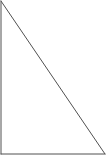
\includegraphics{EgStageI.png} \\
      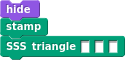
\includegraphics{SSSstampBlank.png} & 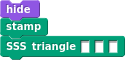
\includegraphics{SSSstampBlank.png} \\
      \hline\hline
      &  \\
      
\includegraphics{EgStageIII.png} & 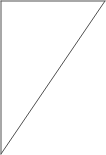
\includegraphics{EgStageIV.png} \\
      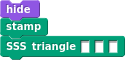
\includegraphics{SSSstampBlank.png} & 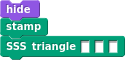
\includegraphics{SSSstampBlank.png} \\\hline
    \end{tabular}
  \end{center}
  The STAMP block records where the turtle starts. As a gesture of
  friendship, I point out that this is a $(104, 153, 185)$ right
  triangle. As usual, you'll need to show your SCRIPTS and STAGES.
  \begin{freeResponse}
    Here they are:
    \begin{center}
    \begin{tabular}{|c||c|}\hline
      &  \\
      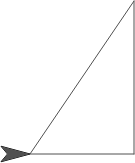
\includegraphics{SSSstampStageII.png} & 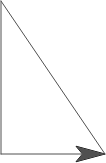
\includegraphics{SSSstampStageI.png} \\
      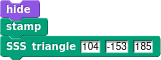
\includegraphics{SSSstampScriptII.png} & 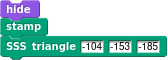
\includegraphics{SSSstampScriptI.png} \\
      \hline\hline
      &  \\
      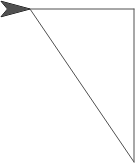
\includegraphics{SSSstampStageIII.png} & 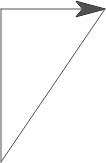
\includegraphics{SSSstampStageIV.png} \\
      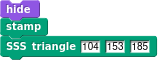
\includegraphics{SSSstampScriptIII.png} & 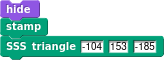
\includegraphics{SSSstampScriptIV.png} \\\hline
    \end{tabular}
  \end{center}
  \end{freeResponse}
\end{question}
\mynewpage

\begin{question}%% SAS
  Demonstrate how to use \raisebox{-.4\height}{
\includegraphics{SASblank.png}} by filling in the
  blanks in the table below.
  \begin{center}
    \begin{tabular}{|c||c|}\hline
      &  \\
      
\includegraphics{EgStageII.png} & 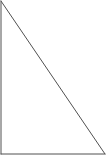
\includegraphics{EgStageI.png} \\
      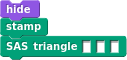
\includegraphics{SASstampBlank.png} & 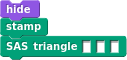
\includegraphics{SASstampBlank.png} \\
      \hline\hline
      &  \\
      
\includegraphics{EgStageIII.png} & 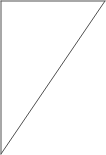
\includegraphics{EgStageIV.png} \\
      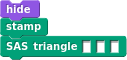
\includegraphics{SASstampBlank.png} & 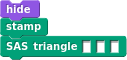
\includegraphics{SASstampBlank.png} \\\hline
    \end{tabular}
  \end{center}
  The STAMP block records where the turtle starts. As a gesture of
  friendship, I point out that this is a $(104, 153, 185)$ right
  triangle. As usual, you'll need to show your SCRIPTS and STAGES.
\end{question}
\mynewpage

\begin{question}%% ASA
\end{question}
\mynewpage

\begin{question}%% SAA
\end{question}
\mynewpage

\begin{question}%% STAIRS
\end{question}
\mynewpage


\end{document}
